\chapter{Desarrollo hardware del manipulador}
\label{cap:capitulo5}

\vspace{1cm}

En este capítulo se aborda el desarrollo necesario para, a partir de un concepto, acabar construyendo un prototipo real funcional. Se 
hace incisión en cada etapa necesaria para este cometido.

\section{Eligiendo la geometría del manipulador}
\label{sec:eligiendo_geometría}
En esta sección se expone como es el proceso de encontrar y definir la forma y funcionamiento del robot, en función de 
los objetivos propuestos, evaluando las distintas opciones para encontrar el que mejor se adapte.  


Primero de todo, se comenzar estableciendo el número de grados de libertad. Esto número esta limitado por los requisitos 
establecidos en la sección \ref{sec:requisitos}. En base a los requisitos 1 y 5, que limitan en cuanto a precio de fabricación y 
complejidad de los mismos, se ha optado por usar 3 grados de libertad.\\

En relación al espacio tridimensional, este cuenta con 6 \acs{DOF}, 3 de ellos para el 
posicionamiento (X, Y, Z) y los otros 3 para las orientaciones (RX, RY, RZ).

\begin{figure} [ht!]
  \begin{center}
    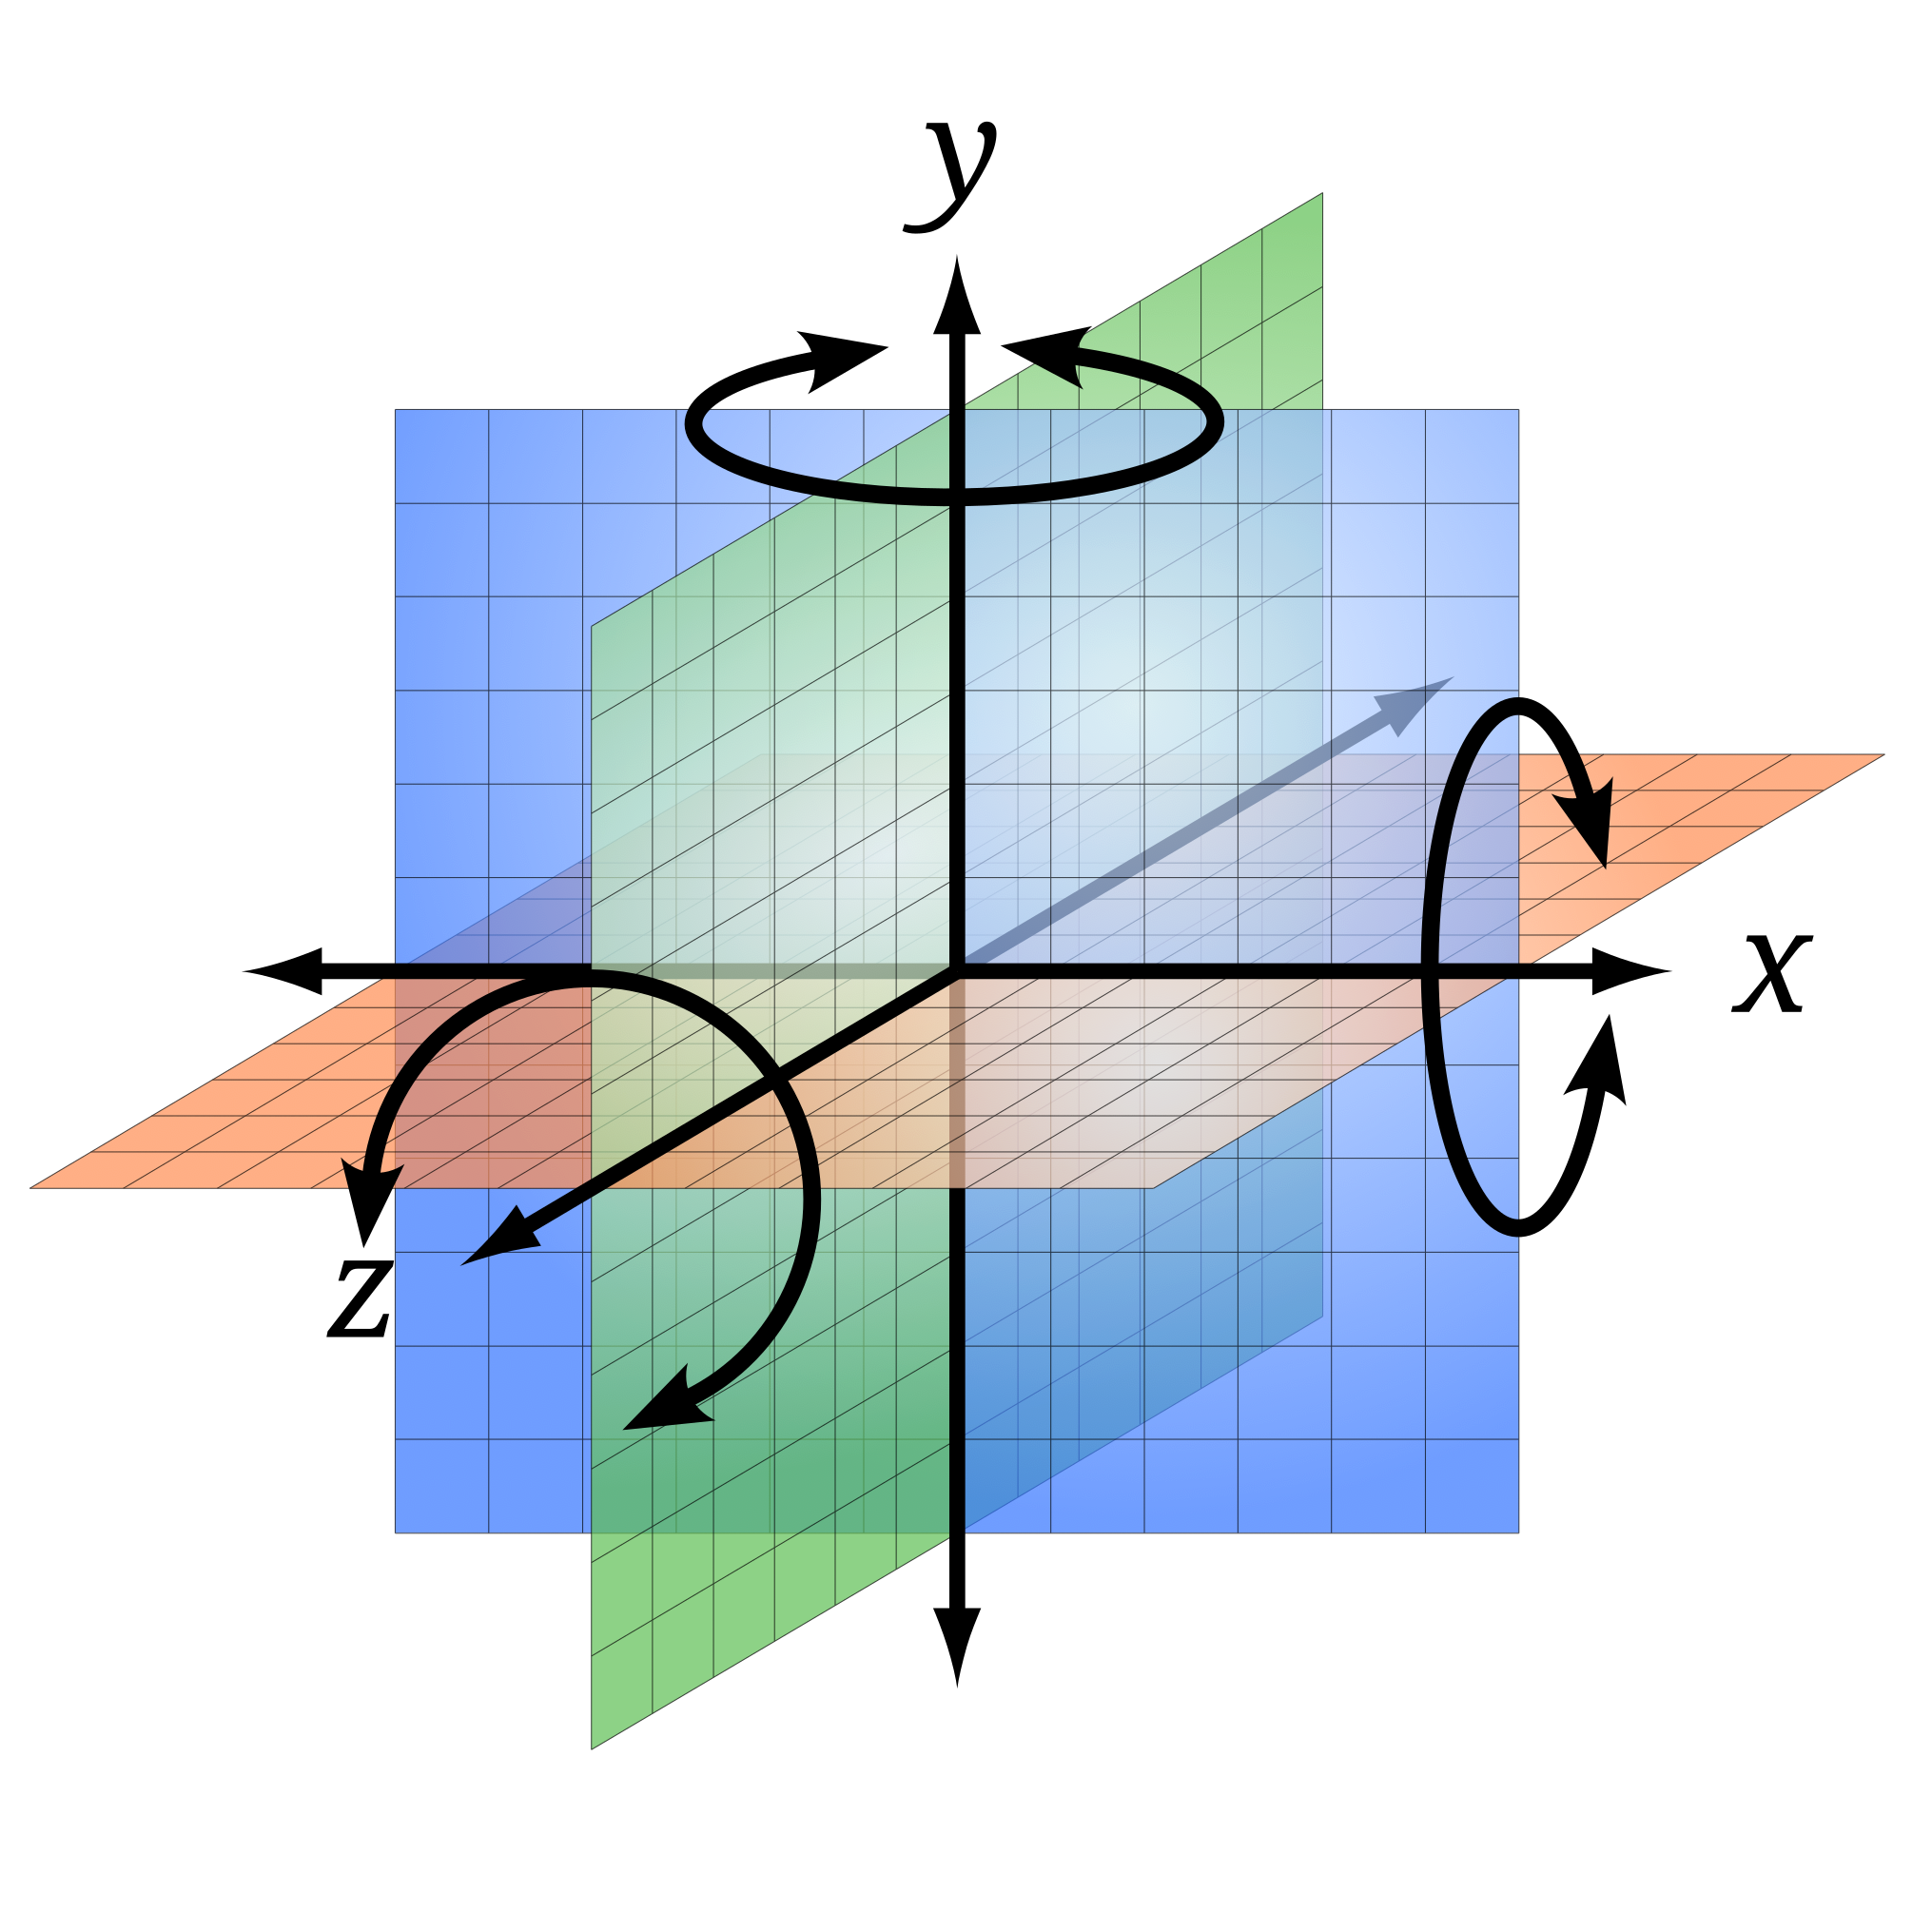
\includegraphics[width=5cm]{figs/coordinates.png}
  \end{center}
  \caption{Espacio tridimensional}
  \label{fig:espacio_tridimensional}
\end{figure}\ 

En base a lo anterior, con 3 grados de libertad no podremos situar el elemento terminal del manipulador en un punto del espacio 
y a la vez controlar la orientación de la herramienta en ese punto.\\

Seguidamente, se debe elegir el tipo de articulación que se pretende usar. En robótica, son ampliamente utilizados estos tipos de 
articulaciones:
\begin{itemize}
\item Revolución: Permite el movimiento de rotación alrededor de un eje fijo.
\item Prismático: Las partes del robot se pueden desplazar linealmente a lo largo de un eje específico. 
\item Esférico: Permite la rotación en cualquier dirección. Está restringido a 3 DOF y suele ser usado como articulación pasiva.
\item Cilíndrica: Permite el movimiento de rotación alrededor de un eje y también un desplazamiento lineal a lo largo del mismo. Combina los movimientos rotacionales y prismáticos. 

\begin{figure} [h!]
  \centering    
  \subfigure[Revolución 1 DOF]{\label{fig:j_rot}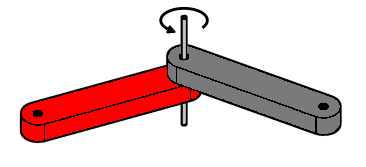
\includegraphics[width=0.3\linewidth ]{figs/joint_rot.png}}
  \hspace{1cm}
  \subfigure[Prismático 1 DOF]{\label{fig:j_prism}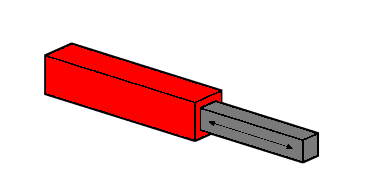
\includegraphics[width=0.3\linewidth]{figs/joint_prism.png}}
  \subfigure[Esférico 3 DOF]{\label{fig:j_esf}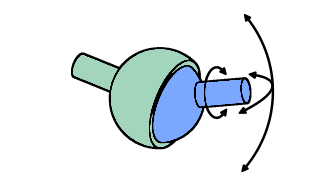
\includegraphics[width=0.3\linewidth ]{figs/joint_esf.png}}
  \hspace{1cm}
  \subfigure[Cilíndrico 2 DOF]{\label{fig:j_cil}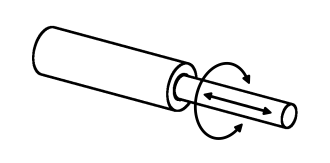
\includegraphics[width=0.3\linewidth]{figs/joint_cil.png}}
  \caption{Tipos de articulaciones más usadas en robótica}
\end{figure}

\end{itemize}

Se ha optado por articulaciones de tipo revolución, debido a que son sencillas de implementar y están compuestas por pocas partes 
móviles.

\newpage
Acto seguido, se debe establecer la forma del manipulador en función del tipo y número de articulaciones elegidas anteriormente. 
En base a las categorías de manipulador descritas en \ref{sec:rob_industrial}, se ha decidido implementar un robot basado 
en paralelogramos al estilo MeArm \ref{fig:mearm}.
\\ 
El tipo de brazo elegido tiene la peculiaridad de tener su elemento terminal siempre paralelo al suelo por lo que es ideal para 
tareas \textit{pick and place}. 

\section{Modelo alámbrico}
\subsection{En qué consiste}
\label{subsec:eqc_mod_alambrico}
El modelo alámbrico es una forma de analizar el movimiento de un sistema mecánico compuesto por ejes y eslabones. Este 
enfoque simplifica la representación visual al destacar las relaciones espaciales entre las diferentes partes del sistema mediante 
líneas y conexiones simbólicas, en lugar de mostrar detalles realistas del manipulador. 
\begin{figure} [ht!]
  \begin{center}
    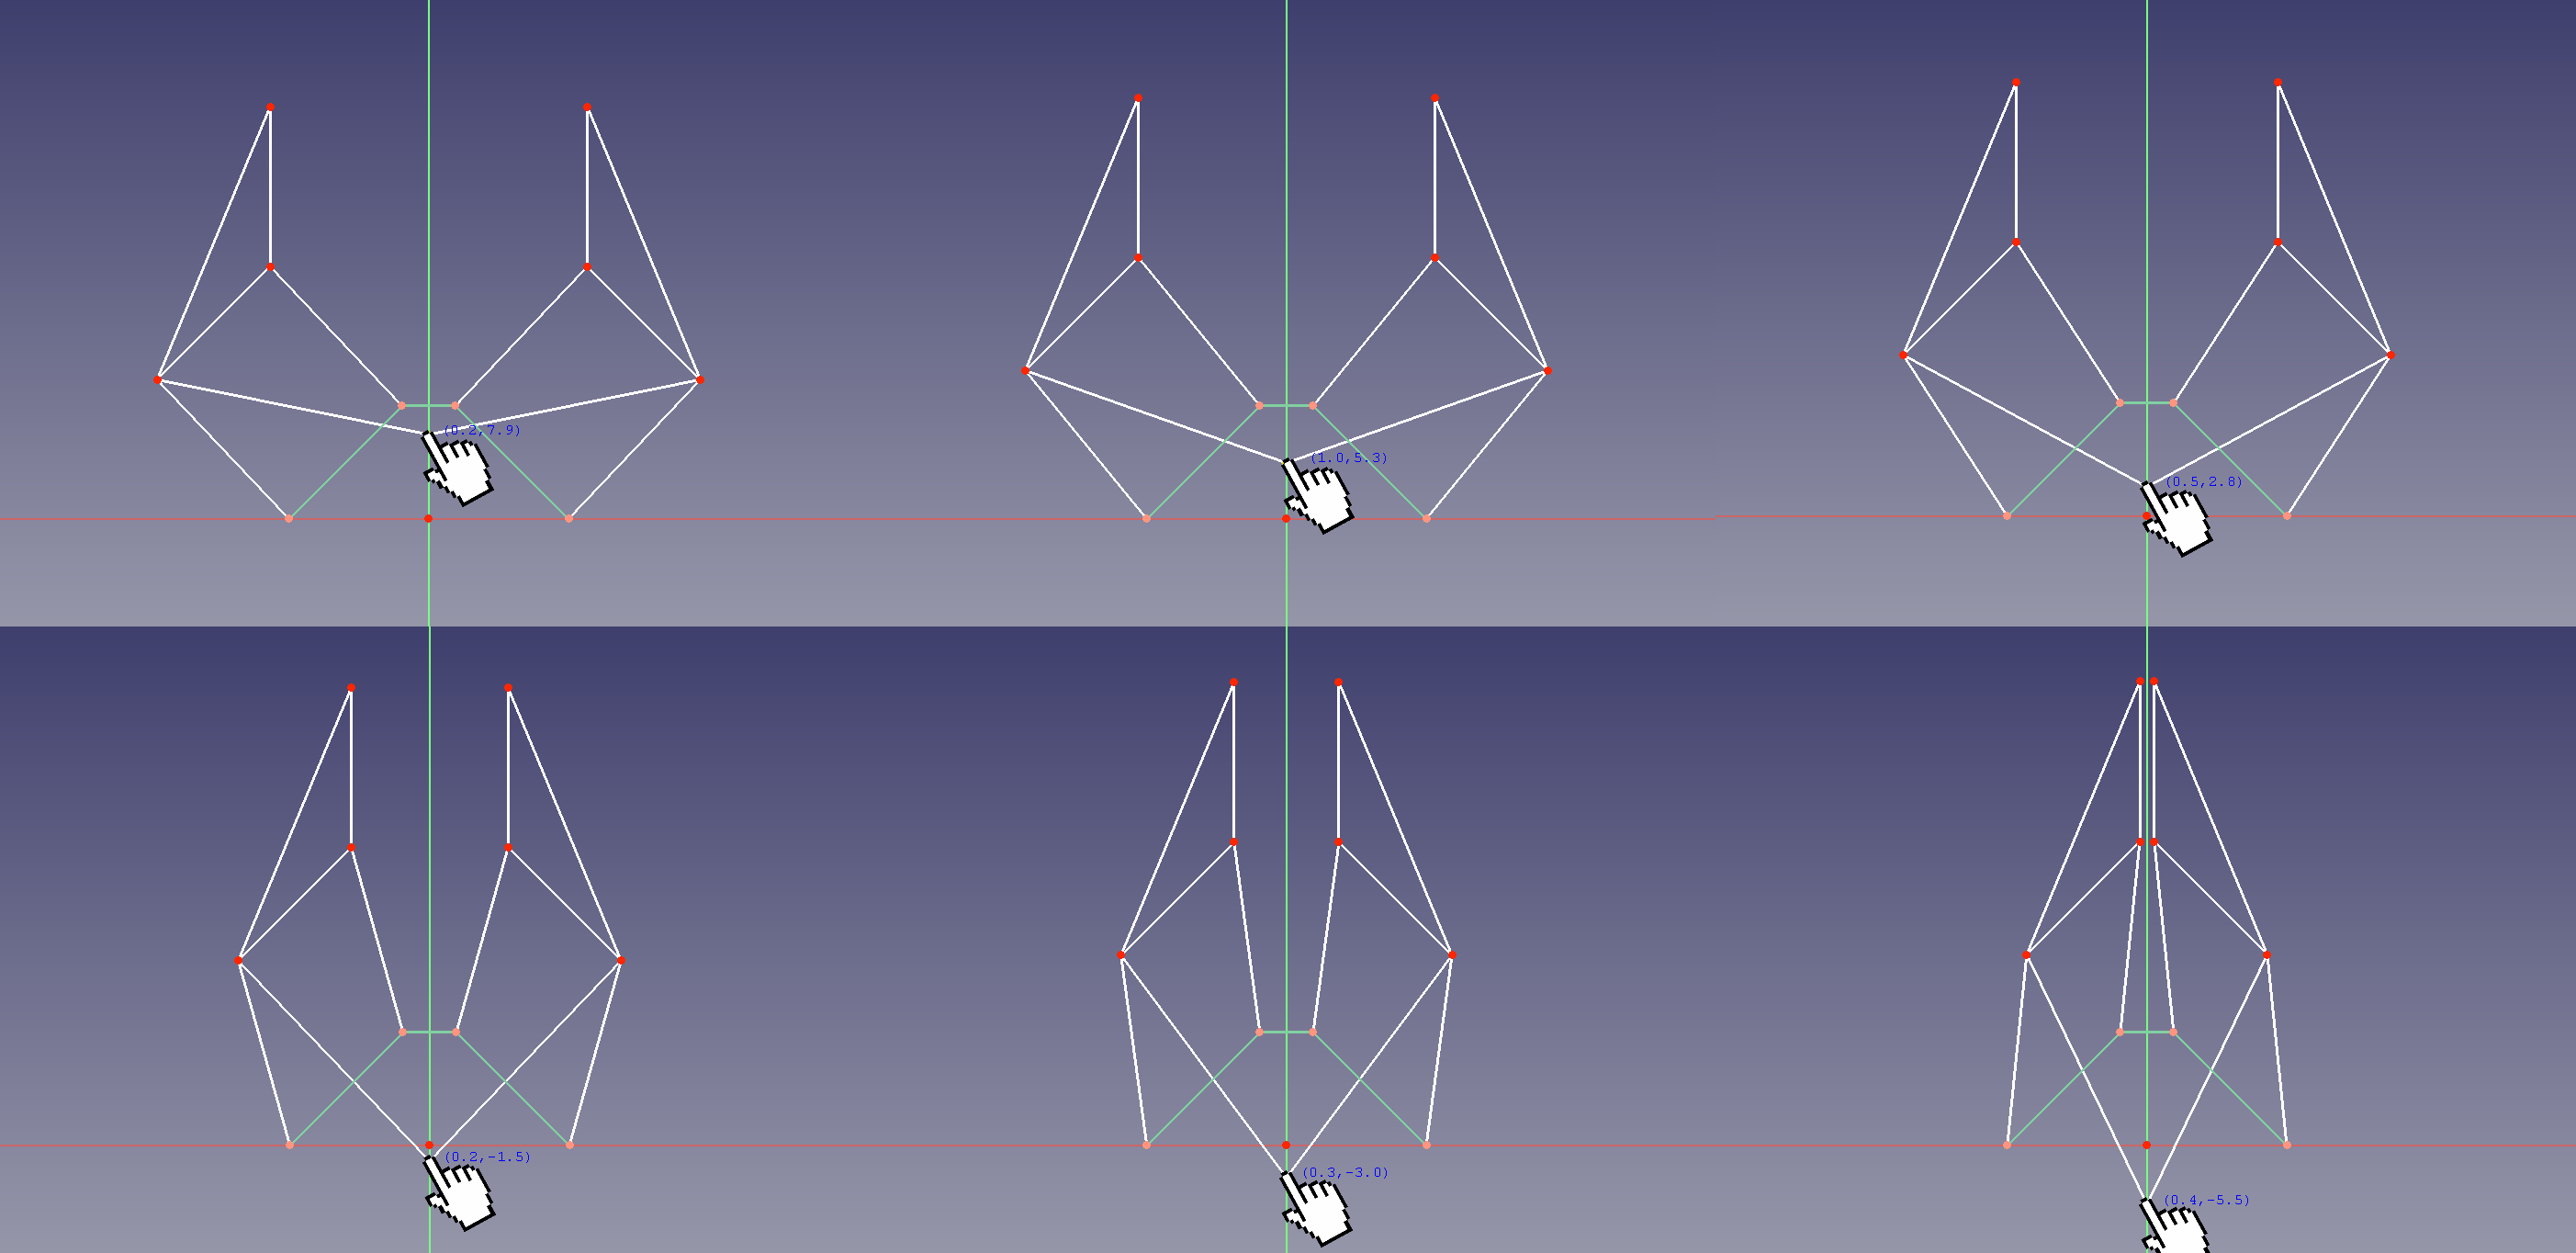
\includegraphics[width=15cm]{figs/pinza_evol.png}
  \end{center}
  \caption{Pinza paralela con 1 grado de libertad}
  \label{fig:mod_pinza_figure}
\end{figure}\ 

\newpage
\subsection{Desarrollo del modelo alámbrico de G-Arm}
\label{subsec:modelo_alambrico}
Para desarrollar el modelo alámbrico de este manipulador, se ha tomado como referencia el modelo alámbrico de MeArm del 
repositorio de github\footnote{\url{https://github.com/myTeachingURJC/Mecatronica/wiki/S3:-Estructuras-mec\%C3\%A1nicas-(II)}}. 
\\
Para abordar adecuadamente la modificación de modelo, es fundamental comprenderlo en su totalidad. Por suerte, el repositorio anterior  
contiene una explicación detallada de la razón de ser de cada elemento.

\begin{figure} [ht!]
  \begin{center}
    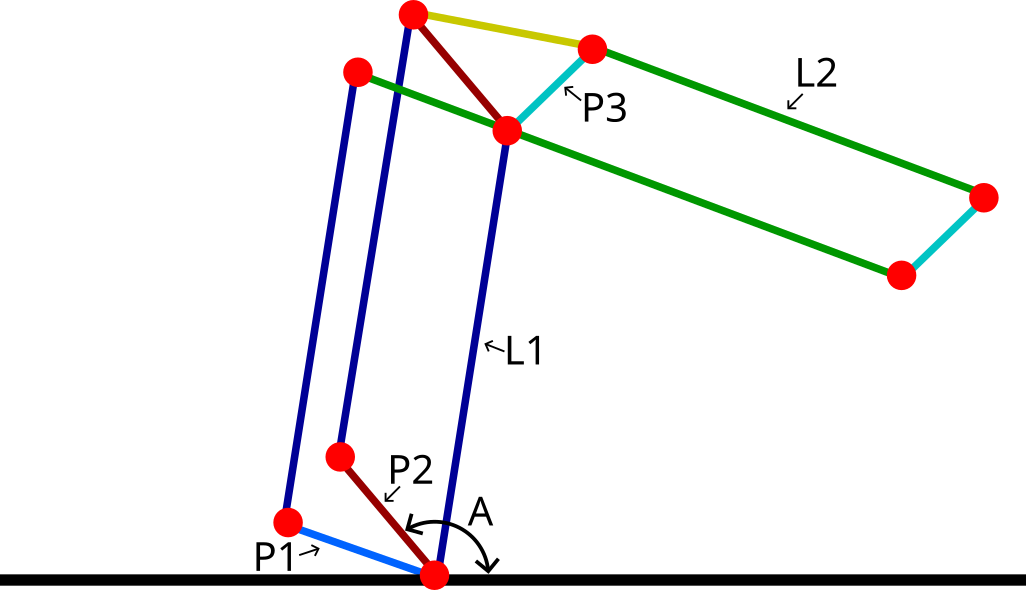
\includegraphics[width=15cm]{figs/mearm_params.png}
  \end{center}
  \caption{Parámetros del modelo alámbrico}
  \label{fig:mod_pinza_figure}
\end{figure}\ 

Este robot está definido por una serie de parámetros (L1, L2, P1, P2, P3, A). Para realizar la obtención de los parámetros que definen a 
G-Arm se ha utilizado la experimentación. El procedimiento ha consistido en modificar una medida y evaluar como se 
comporta a la hora de alcanzar ciertas zonas críticas. El objetivo final es encontrar una combinación de parámetros que 
permita alcanzar la mayor cantidad de puntos sin que sus eslabones intersecten entre sí. 

\newpage
Más concretamente, la obtención de los parámetros adecuados se realizó en el siguiente orden:
\begin{enumerate}
\item Una manera de comenzar, es estableciendo de antemano el largo de los eslabones primarios L1 y L2. En base al peso estimado de 
cada uno de ellos, y de los motores utilizados, ambos deberían medir 17cm o menos.
\item El siguiente paso es elegir P1, P2 y P3. Estos son los lados cortos del los paralelogramos. Es importante jugar con estos valores 
de tal manera que se consiga obtener los más largos posibles. Esto es debido a que las piezas reales ocupan un cierto espacio y si el paralelogramo es 
muy pequeño no realizarán todo el recorrido ya que chocarán entre sí. Codo
\item El ángulo A restringe el paralelogramo que mantiene el extremo del robot paralelo al suelo.   
\end{enumerate}
En esta imagen se muestra el modelo alámbrico de G-Arm:\\
\begin{figure} [ht!]
  \begin{center}
    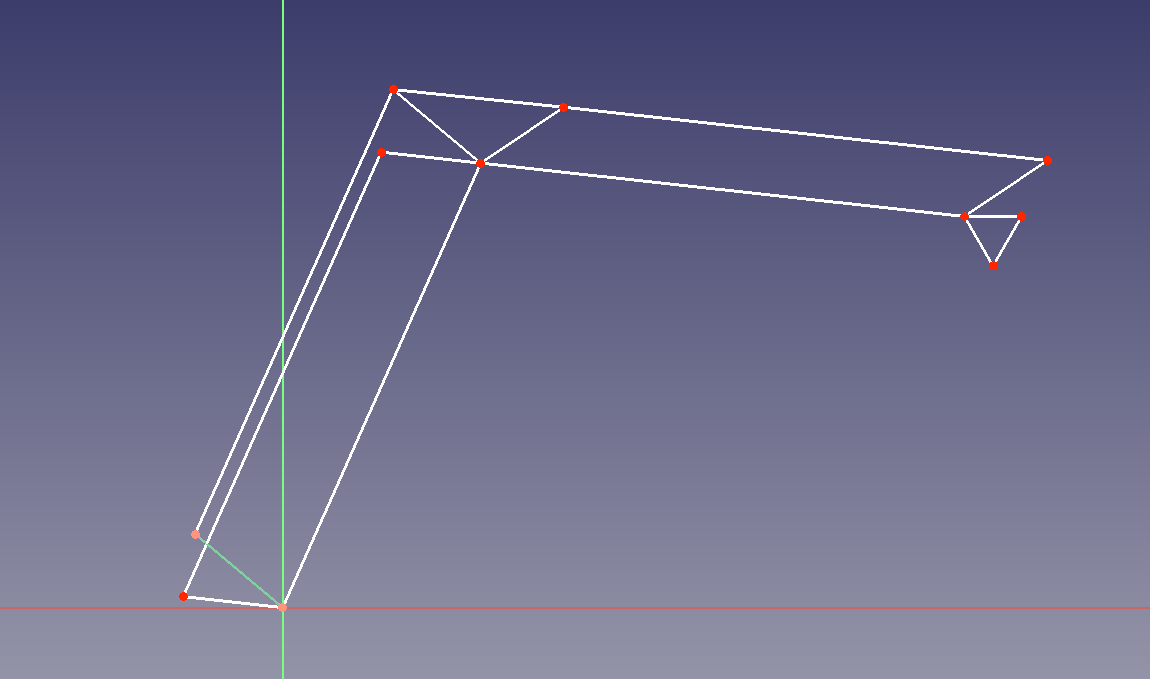
\includegraphics[width=15cm]{figs/alambrico_garm.png}
  \end{center}
  \caption{Modelo alámbrico de G-Arm}
  \label{fig:mod_pinza_figure}
\end{figure}\ 
Revisar parametros
\newpage
En la siguiente tabla se muestran los valores obtenidos: 
\begin{table}[H]
\begin{center}
\begin{tabular}{|c|c|}
\hline
\textbf{Parámetros} & \textbf{Valores} \\
\hline
L1 & 170mm \\
L2 & 170mm \\
P1 & 35mm \\
P2 & 35mm \\
P3 & 25mm \\
A & 135º \\
\hline
\end{tabular}
\caption{Parámetros del modelo alámbrico de G-Arm}
\label{cuadro:parametros_alambrico}
\end{center}
\end{table}

\section{Bocetos}
Una parte importante del diseño son los bocetos previos al modelado 3D. En estos bocetos se busca tener una idea clara de la forma 
y posición de cada pieza, así como de su lugar en el espacio.  
Para el desarrollo de este brazo, se han realizado numerosos bocetos, de los cuales se conservan aquellos dibujados digitalmente por medio 
de un iPad.
\section{Elección de componentes hardware}
En esta sección se analiza las necesidades que deben satisfacer los componentes hardware (motores, placas, fuentes de alimentación etc.)
y se busca la mejor opción rendimiento-precio existente en el mercado. 

\subsection{Motores}
Según la geometría establecida en \ref{sec:eligiendo_geometría}, el robot necesita 3 motores. Los utilizados en este proyecto deben
cumplir las siguientes características:
\begin{enumerate}
  \item Deben ser capaces de entregar el suficiente torque para levantar el brazo más una cierta la carga en su extremo.
  \item Se debe poder conocer su posición en cada instante.
  \item Deben poder mantener su torque sin estar en movimiento.
\end{enumerate}

Debido a esta última necesidad, no es buena idea usar motores convencionales de corriente contínua con escobillas, ya que no son 
capaces de aportar torque sin girar. Por otro lado, los motores paso a paso si son capaces de ello y, aunque no estén codificados,
se puede conocer la posición relativa ya que avanza en pequeños incrementos discretos (pasos). Además, este tipo de motor es capaz de 
entregar un torque considerable para su tamaño. Por contra, son bastante pesados. 

Tras investigar las opciones existentes en el mercado, se ha llegado a la conclusión que los motores Nema 17 son la opción ideal 
para la realización de este trabajo debido a que son comunes y fáciles de encontrar, además de tener un precio aceptable. Aún así, 
existen motores Nema de diferentes tamaños, para realizar robots más o menos grandes.
\begin{figure} [ht!]
  \begin{center}
    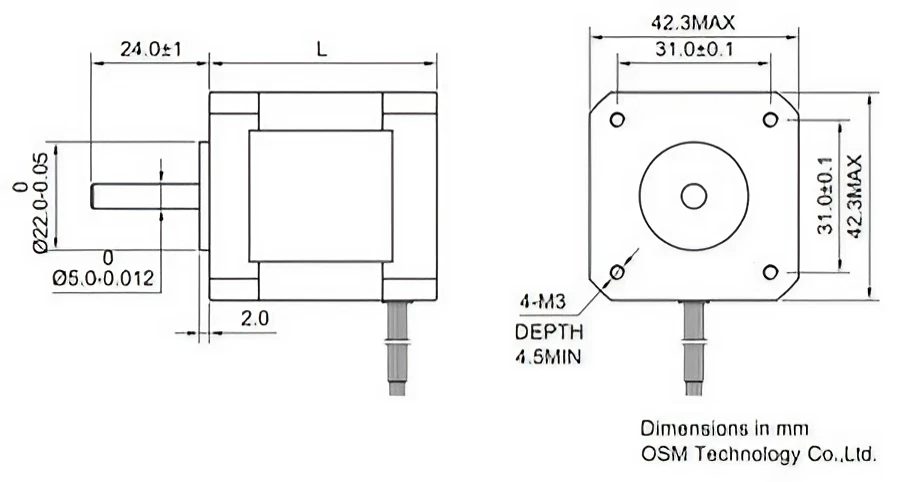
\includegraphics[width=15cm]{figs/MotorsNema.png}
  \end{center}
  \caption{Diferentes categorías de motor paso a paso Nema \footnote{\url{https://filament2print.com/es/blog/139_motores-nema.html}}}
  \label{fig:nema}
\end{figure}\ 

Dentro de la categoría Nema 17, todos tienen el mismo factor de forma a excepción del largo del motor. Esta característica determina 
el torque del motor. A mayor longitud, mayor torque es capaz de ejercer. 

Fotito de lo necesario

\subsection{Reductora}
Para poder reducir la velocidad de giro de un motor y, a su vez convertirla en fuerza, es necesario la implementación de una reductora. 
Existen diferentes formas de hacerlo, como pueden ser los engranajes (normales, planetarios, helicoidales...) y las correas (lisas y 
dentadas).

Se ha optado por el uso de correas dentadas sobre el uso de engranajes debido a que estos últimos siempre añaden una cierta holgura 
al movimiento final, haciendo el robot inexacto y añadiendo incertidumbre en los movimientos. Las correas dentadas en cambio, utilizan 
tensores para asegurar que siempre está en contacto con ambas poleas.

Foto de correa dentadas
Se pretenden usar correas de tipo GT2. Este tipo de correa es ampliamente utilizado en impresoras 3D, por lo que es realmente económico y 
fácil de encontrar. Dentro de esta categoría existen diferentes anchos de correa en función de la tensión soportada. En este caso, 
se ha elegido el ancho de 6mm puesto que es el más económico con diferencia y más que suficiente para esta aplicación. En la construcción 
de robot industriales caseros y profesionales de metal y de gran tamaño, se utilizana correas y cadenas con mayor grosor y tamaño de diente.
Foto de mi correa.

\subsection{Controladores}
Debido a que se prentende utilizar motores paso a paso bipolares, es necesario utilizar controladores de motores paso a paso. 
xiste un formato y estas opciones

\subsection{Placa base}
La placa base es una targeta de circuito impreso que proporciona conexiones físicas y eléctricas entre las diferentes componentes y 
unifica estos en un mismo componente. 
En el caso de aquellas usadas para montar controladores paso a paso, suelen integrar un \ac{MCU} o actuar como un \textit{shield} 
(placa adicional que se acopla a otras para aumentar su funcionalidad y características).
Foto cnc arduino shield y otras

Existen numerosas opciones en el mercado con la posibilidad de montar una distinta cantidad de controladores. En el caso de este 
trabajo necesitamos sólamente 3. Este tipo de placas suelen ser utilizadas para crear máquinas CNC y en este caso se ha optado por 
elegir una placa económica que integra todo lo necesario para este proyecto a exccepción de los controladores. 
Se ha elegido esta y no otra puesto que tiene un \acs{MCU} ESP32 muy superior al AtMega328p del Arduino Uno. Además cuenta con la 
capacidad de poderse controlar vía wifi y la mayor ventaja es que incorpora un mosfet conectado a una salida pwm a la que podemos conectar 
un motor de hasta x vatios, un electroimán etc. Además incluye una serie de pines y salidas muy cónmodas de utilizar para montar 
módulos de grabado láser y etc. Todo ello por un precio de 16€.

\subsection{Fuente de alimentación}
Un elemento clave de un sistema electrónico es la fuente de alimentación. Es importante conocer \textit{a priori} las 
características necesarias de la fuente.

Los motores Bla
La placa es capaz de trabajar en un rango de 12 a 24v 
el consumo tal
\subsection{Rodamientos}
Para mejorar la eficiencia de las articulaciones y garantizar que todas roten con suavidad, se pretende hacer uso de rodamientos 
en cada una de ellas. 
Existen diferentes tipos de rodamientos en el mercado pero se ha elegido un tipo de rodamiento específico para este propósito. 
Se ha optado por el uso de rodamientos brida. Este tipo de rodamientos son usados en las poleas pasivas de las impresoras 3D, por lo 
que son muy baratos (10 de buena marca por 6-10€) y sencillos de encontrar. La razón principal de su uso es su peculiar forma. Este tipo 
de rodamiento tiene un borde en el extremo que hace de borde. esto lo hace ideal para insertar en las piezas 3d a desarrollar y garantizar 
que nunca se puedan sacar mientras el tornillo este fijado. Además evita que el rodamiento se mueva y se gire cuando la articulación 
recibe un esfuerzo lateral. 

\begin{figure} [ht!]
  \begin{center}
    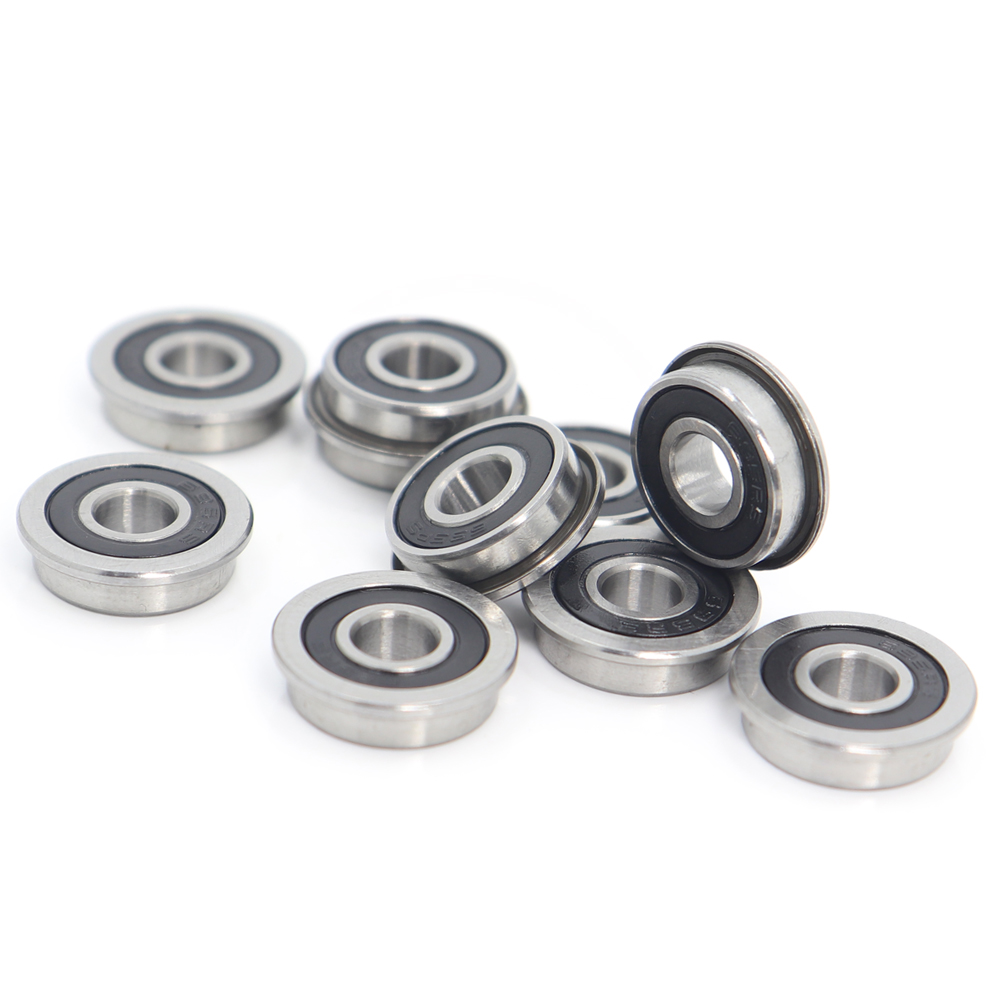
\includegraphics[width=10cm]{figs/F695-2RS.jpeg}
  \end{center}
  \caption{Rodamientos F695-2RS Fushi \footnote{\url{https://es.aliexpress.com/item/32850989216.html}}}
\end{figure}\ 



\subsection{Finales de carrera}
\newpage
\section{Diseño CAD}
En esta sección se va a hablar de las particularidades del diseño y diversas cosas que hay que tener en cuenta a la hora de diseñar 
cualquier pieza mecánica que posteriormente será impresa en plástico. 
\\
Para el diseño de este brazo robot, se ha utilizado dos herramientas de diseño. Inicialmente el proyecto se realizó mediante 
la herramienta \textit{Fusion 360} y posteriormente se utilizó FreeCad\ref{sec:freecad} para cumplir el objetivo de ser totalmente 
\textit{Open Source} y parametrizado, para que cualquier persona pueda investigarlo, modificarlo y utilizarlo de forma gratuita.
\\ 
El diseño 3D se ha ido contruyendo a partir de los bocetos y modificando ligeramente en función de como iba quedando.

pruebas que hice

\newpage
\section{Impresión y montaje}
En esta sección se exponen todos los detalles a tener en cuenta a la hora de querer replicar este proyecto. Para la impresión 
de G-Arm se ha utilizado una impresora Ender-3 Pro\footnote{\url{https://www.creality.com/products/ender-3-pro-3d-printer}} y un rollo 
de 1Kg de filamento PLA Rojo convencional.
\begin{figure} [h!]
\begin{center}
  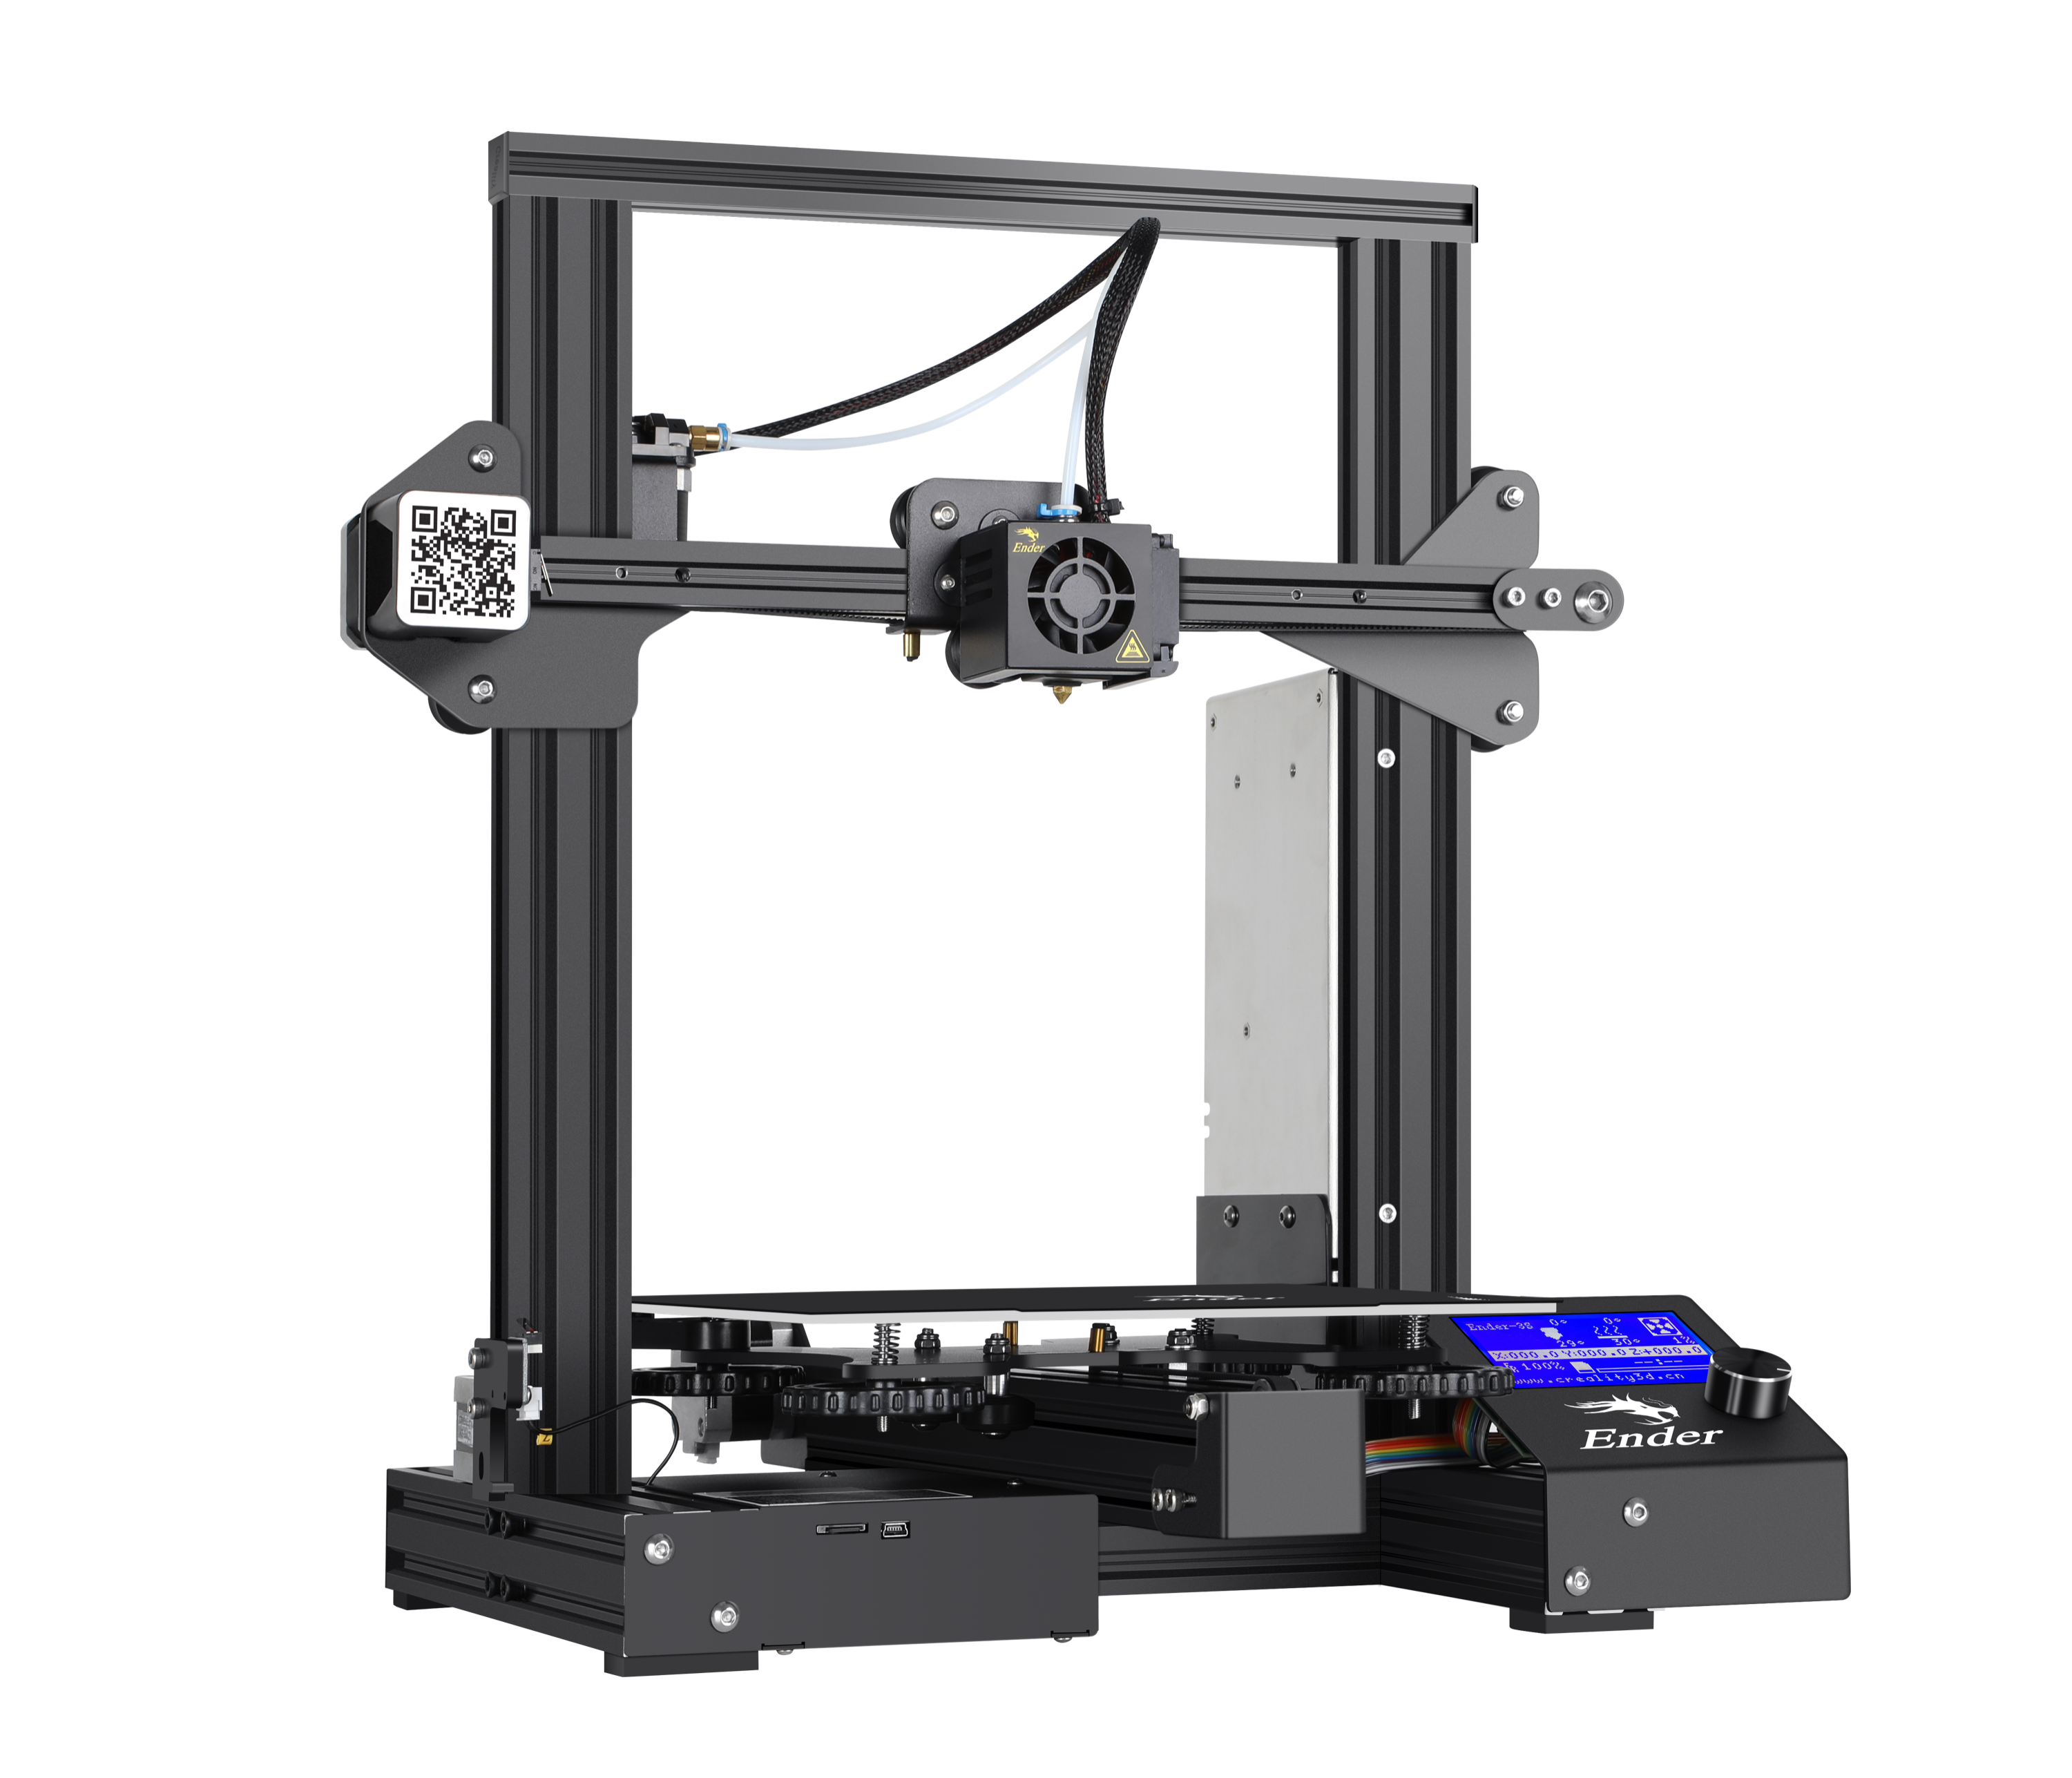
\includegraphics[width=8cm]{figs/ender3.png}
\end{center}
\caption{Ender-3 Pro V1 2017}
\label{fig:ender3pro}
\end{figure}\   

\begin{table}[H]
\begin{center}
\begin{tabular}{|c|c|c|c|}
\hline
\textbf{Componente} & \textbf{Modelo} & \textbf{Cantidad} & \textbf{Precio total} \\
\hline
Motor Nema 17 & 17HS24-2104S & 3 & 56\euro \\
Controlador & TMC2209 & 3 & 10\euro \\
Placa base & MKS DLC32 & 1 & 16\euro \\
Final de carrera & MakerBot (rojo) & 3 & 5\euro \\
Fuente de alimentación & 24V 5A (opcional)\ref{subsec:fuente_alimentacion} & 1 & 15\euro \\
Rodamiento &  F695-2RS Fushi & 22 & 15\euro \\
Rodamiento & F623RS Fushi & 6 & 5.5\euro \\
Polea GT2 & Correa:6mm ID:5mm & 3 & 1.5\euro \\
Correa GT2 & Correa:6mm Largo:252mm & 2 & 3.5\euro \\ 
Correa GT2 &  Correa:6mm Largo:280mm & 1 & 1.8\euro \\ 
Ventilador & 24V 4010 & 1 & 2\euro \\
Electroimán & D20H15mm 3KG 24V & 1 & 3\euro \\
Plástico para imprimir & PLA/PETG 1Kg & 1 & 22\euro \\
\hline
\end{tabular}
\caption{Componentes hardware necesarios}
\label{cuadro:componentes}
\end{center}
\end{table}

\begin{table}[H]
\begin{center}
\begin{tabular}{|c|c|c|}
\hline
\textbf{Componente} & \textbf{Cantidad} & \textbf{Precio total} \\
\hline
Tornillo M3 Allen & 3 & 56\euro \\

\hline
\end{tabular}
\caption{Tornillería necesaria}
\label{cuadro:tornilleria}
\end{center}
\end{table}

El precio total de los componentes necesarios es: 156.3\euro
\begin{table}[H]
\begin{center}
\begin{tabular}{|c|c|c|}
\hline
\textbf{Identificador} & \textbf{Cantidad} & \textbf{Relleno óptimo} \\
\hline
\#1 & 1 & 15\% \\
\hline
\end{tabular}
\caption{Piezas necesarias}
\label{cuadro:piezas}
\end{center}
\end{table}

